\subsubsection{算法类别}
Dijkstra单源最短路径算法属于贪心算法.

\paragraph{问题描述}
给定带权有向图$G=(V,E)$, 其中每条边的权是\textbf{非负实数}. 另外, 还给定V中的一个顶点,
称为源. 现在要计算从源到所有其他各顶点的最短路长度.
此处的最短路长度指路上各边权之和. 这个问题通常称为\textbf{单源最短路径问题}.

\paragraph{Dijkstra算法的基本思路}
求解的基本思路是, 设置顶点集合S并不断地进行贪心选择来扩充这个集合.
一个顶点属于集合S当且仅当从源到该顶点的最短路径长度已知.\par

初始的时候, S中仅含有源. 设u是G的某一个顶点,
把从源到u且中间只经过S中顶点的路称为从源到u的特殊路径,
并记录当前每个顶点所对应的最短特殊路径长度.
Dijkstra算法每次从V-S中取出具有最短特殊路径长度的顶点u, 将u添加到S中,
同时更新影响到的顶点所对应的最短特殊路径长度. 一旦S中包含了所有V中的顶点,
就已经完成了从源到其他顶点之间的最短路径长度.

\paragraph{单源最短路径问题的的最优子结构性质}
对图$G(V, E)$, 源点v, 问题从以下三方面描述:
\begin{enumerate}
	\item 源点v, 途中顶点集合V在算法的迭代过程中均保持不变;
	\item 用于构造最短路径的当前顶点集合$S_i$, 不断增加, 定义不同规模的子问题;
	\item 指标: 相对于现有的$S_i$, 对各顶点u, 记录其到源点的距离u.distance.
\end{enumerate}

不同的$S_i$, 定义了不同规模的子问题; 当$S_i = V$的时候, 算法迭代结束,
此时$u.distance, \every u \in V$表示途中任意顶点到源的距离.\par

对越小的$S_i$, 问题越简单, 故自下而上求解.

\paragraph{Dijkstra算法的贪心选择性质}
\begin{description}
	\item[贪心选择策略] 在每步迭代的时候, 从$V-S$
		中选择具有最短特殊路径u.dist的顶点u, 加入S.
	\item[贪心策略的正确性] 需要证明对顶点u, 从v开始,
		经过G中任意顶点到达u的全局最短路径长度$d(v, u) = u.dist$,
		其中u.dist是从v开始, 只经过S中的顶点到达u的最短路径.
		即不存在另一条v到u的最短路径, 使得其中某些节点在$V-S$中,
		且该路径的长度$d(v, u)< u.dist$.
\end{description}

\subsubsection{关键函数及代码段的描述}
其伪代码描述如下:
\begin{algorithm}
	\caption{Dijkstra's algorithm}\label{alg:dijkstra}
	\begin{algorithmic}{1}
		\Require $(G, w, s)$
		\State $S = \emptyset$
		\State $Q = G.V$
		\While{$Q \neq \emptyset$}
		\State $u = Extract-Min(Q)$
		\State S = S \cup \{u\}
		\For{$each vertex v \in G.Adj[u]$}
		\State Relax(u, v, w)
		\EndFor
		\EndWhile
	\end{algorithmic}

	\begin{algorithmic}{1}
		Require $(u, v, w)$
		\If{$v.d > u.d + w(u, v)$}
		\State $v.d = u.d + w(u, v)$
		\EndIf
	\end{algorithmic}
\end{algorithm}

其核心代码实现如下:

\begin{lstlisting}[language=c++]
void BackPack01::backPackDP() {
    maxVal = -1;

    // Initialize
    for (int j = 0; j <= volume; j++) {
        dp[n - 1][j] = (j >= w[n - 1]) ? val[n - 1] : 0;
    }

    int i = n - 2, j = volume;
    for (; i >= 0; i--) {
        j = volume;
        for (; j >= 0; j--) {

            // Compare total value of items in the backpack between put
            // item[i] in and not put it in.
            dp[i][j] = (j >= w[i]) ? std::max(dp[i + 1][j],
                                              dp[i + 1][j - w[i]] + val[i])
                                   : dp[i + 1][j];
        }
    }

    maxVal = dp[0][volume];
}
\end{lstlisting}

\subsubsection{算法时间及空间复杂性分析}
\paragraph{空间复杂度分析}
0-1背包问题的动态规划实现需要一个大小为N*C的数组进行辅助,
所以空间复杂度为$O(NC)$.

\paragraph{时间复杂度分析}
由于动态规划的本质是上述递推式\ref{eq:01bp-sub-problem},
且实现的核心代码使用了两层循环, 所以可以很方便的计算出时间复杂度为

\begin{equation}
	C(n) = O(N)\times O(C) = O(NC)
\end{equation}

% \begin{gather}
% 	C'(0) = 0            \nonumber \\
% 	C'(k) = 2C'(k-1)+2^k \nonumber
% \end{gather}
综上, 0-1背包问题的一般动态规划解法的时间复杂度为O(NC).

\subsection{应用跳跃点方法优化的0-1背包问题动态规划解法}
\subsubsection{算法类别}
应用了跳跃点方法优化的0-1背包问题解法也是一种动态规划方法.

\subsubsection{算法思路}
\label{sec:jumpPointThink}
\paragraph{概述}
由$m(i, j)$的递归式容易证明, 在一般的情况下, 对每一个确定的$i(1\leq i\leq n)$,
函数$m(i, j)$是关于变量j的阶梯状单调不减函数. 跳跃点是这一类函数的描述特征.
在一般情况下, 函数$m(i, j)$由其全部跳跃点唯一确定. 如图所示.

\begin{figure}[ht!]
	\centering
	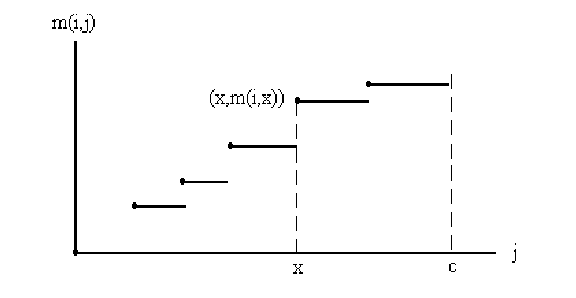
\includegraphics[width=0.8\textwidth]{figures/JumpPoint.png}
	\caption{跳跃点}
	\label{fig:JumpPoint}
\end{figure}

对每一个确定的$i,(1\leq i\leq n)$, 用一个链表p[i]存储函数$m(i,j)$的全部跳跃点.
链表p[i]可以计算$m(i,j)$的递归式递归地由表p[i+1]计算,
初始的时候p[n+1]=\{(0,0)\}.

\paragraph{算法改进的描述}
函数$m(i,j)$是由函数$m(i+1,j)$与函数$m(i+1, j-w_i)+v_i$作max运算得到的. 因此,
函数$m(i,j)$的全部跳跃点包含于函数$m(i+1,j)$的跳跃点集p[i+1]与函数
$m(i+1,j-w_i)+v_i$的跳跃点集q[i+1]的并集中.\par

易知, $(s,t)\in q[i+1]$当且仅当$w_i\leq s\leq c$且$(s-w_i,t-v{i})\in p[i+1]$. \par

因此, 容易由p[i+1]确定跳跃点集q[i+1]如下:
\begin{equation}
	q[i+1]=p[i+1]\oplus (w_i,v_i)=\{(j+w_i,m(i,j)+v_i)|(j,m(i,j))\in p[i+1]\}
	\label{eq:jumpSet}
\end{equation}

另一方面, 设(a,b)和(c,d)是$p[i+1]\cup q[i+1]$中的2个跳跃点, 则当$c\geq
	a$且$d<b$的时候, (c,d)受控于(a, b), 从而(c, d)不是p[i]中的跳跃点.
除了受控跳跃点之外, $p[i+1]\cup q[i+1]$中的其他跳跃点都是p[i]中的跳跃点.\par

由此可见, 在递归地由表p[i+1]计算表p[i]的时候, 可以先由p[i+1]计算出q[i+1],
然后合并表p[i+1]和表q[i+1], 并清除其中的受控跳跃点得到表p[i].

\subsubsection{关键函数及代码段的描述}
使用跳跃点优化的动态规划方法求解0-1背包问题的关键在于根据上述推导过程动态
根据上一状态的跳跃点集维护当前状态的跳跃点. 具体代码如下:\par
对函数均使用类似C++的Pseudo-Code描述.

\begin{lstlisting}[language=c++]
void BackPackJumpPoint::JumpPointBackPackDP() {
    int *head = new int[n + 2]; // Track jump point start position.
    head[n] = 0;
    jp[0][0] = 0; // Store item weight
    jp[0][1] = 0; // Store item value

    // Left points to first jump point of p[i+1], right points to last jump
    // point of p[i+1]. Next is position where next jump point will store.
    int left = 0, right = 0, next = 1;
    head[n - 1] = 1; // Points to the position of first jump point of item[n-1].

    for (int i = n - 1; i >= 0; i--) {
        int k = left; // k points to jump points of p[], move k to
                      // evaluate controlled points in p[] and
                      // p[]+(w,v)
        for (int j = left; j <= right; j++) {

            if (jp[j][0] + w[i] > volume) {
                // No enough backpack space to fit item[i] in, exit loop.
                break;
            }

            // Compute new jump point as jp[]+(w,v).
            int x = jp[j][0] + w[i];
            int y = jp[j][1] + val[i];

            // If jp[k][0] < x, then it must be a jump point of current
            // item.
            while (k <= right && jp[k][0] < x) {
                jp[next][0] = jp[k][0];
                jp[next++][1] = jp[k++][1];
            }

            // Clear controlled jump point.
            if (k <= right && jp[k][0] == x) {
                if (y < jp[k][1]) {
                    y = jp[k][1];
                }
                k++;
            }

            if (y > jp[next - 1][1]) {
                jp[next][0] = x;
                jp[next++][1] = y;
            }

            while (k <= right && jp[k][1] <= jp[next - 1][1]) {
                k++;
            }
        }

        // Add remaining jump points.
        while (k <= right) {
            jp[next][0] = jp[k][0];
            jp[next++][1] = jp[k++][1];
        }

        left = right + 1;
        right = next - 1;

        head[i - 1] = next;
    }


    maxVal = jp[next - 1][1];
}
\end{lstlisting}

\subsubsection{算法时间及空间复杂性分析}
\paragraph{空间复杂度分析}
在我的C++版和Rust版实现中, 均采用了邻接表数据结构,
表示具有n个顶点和e条边的带权有向图$G(V, E)$. 在平均情况下, 空间复杂度为$O(V+E)$;
在最坏情况下, 空间复杂度为$O(V^2)$.\par

相比于一般的邻接矩阵表示方式, 邻接表方式在绝大多数情况下所需空间都更少.

\paragraph{时间复杂度分析}


从而, 改进后算法的计算时间复杂性为$O(2^n)$. 当所给物品的重量$w_i(1\leq i\leq n)$
是整数的时候, $|p[i]|\leq c+1, (1\leq i\leq n)$. 在这种情况下,
改进后的算法的计算时间复杂度为$O(min\{nc, 2^n\})$.

% \begin{align}
% 	C(1)       & = 0                        \nonumber \\
% 	C_{min}(n) & = 2C(\frac{n}{2}) + n - 1  \nonumber \\
% 	C_{max}(n) & = C(1) + C(n - 1) + n - 1  \nonumber
% \end{align}
